\documentclass{article}
\usepackage{graphicx}
\usepackage{booktabs}
\usepackage{amsmath}
\usepackage{geometry}
\geometry{a4paper, margin=1in}

\title{Simple Analysis of a CNN-SVM Hybrid for MNIST Digit Recognition}
\author{Written by Haileiyesus Mesafint}
\date{\today}

\begin{document}

\maketitle

\begin{abstract}
This report looks at a small experiment comparing two approaches for classifying handwritten digits from the MNIST dataset. The first is a regular Convolutional Neural Network (CNN). The second uses a CNN to extract features, then a Support Vector Machine (SVM) to do the final classification. The goal is to see if the hybrid approach works better than the standard CNN. The code and results come from the provided Jupyter Notebook.
\end{abstract}

\section{Introduction}
The MNIST dataset is a common benchmark for image classification. CNNs usually perform very well on it. In this experiment, we test whether using a CNN only for feature extraction, followed by an SVM classifier, can match or beat a pure CNN. This report reviews the notebook results and explains the findings.

\section{Method}
We used PyTorch to build and train the CNN, and Scikit-learn for the SVM and evaluation.

\subsection{Data and Preprocessing}
We worked with the standard MNIST dataset: 60,000 training images and 10,000 test images of digits (0–9). Each image was converted to a tensor and normalized with mean 0.1307 and standard deviation 0.3081.

\subsection{Pure CNN Model}
We first trained a regular CNN as a baseline.

\subsubsection{Architecture}
The CNN has two parts: a feature extractor and a classifier.
\begin{itemize}
    \item \textbf{Feature extractor}: 
    \begin{itemize}
        \item Conv1: 1 input channel, 32 output channels, kernel 3$\times$3, padding 1.
        \item MaxPool1: 2$\times$2.
        \item Conv2: 32 input channels, 64 output channels, kernel 3$\times$3, padding 1.
        \item MaxPool2: 2$\times$2.
    \end{itemize}
    \item \textbf{Classifier}: A fully connected layer maps the flattened features to 10 outputs (one per digit). The feature size was 128. Softmax is handled by the loss function.
\end{itemize}

\subsubsection{Training}
The CNN was trained for 6 epochs, batch size 128, learning rate 0.001, Adam optimizer, and Cross-Entropy Loss.

\subsection{CNN-SVM Hybrid Model}
For the hybrid:
\begin{enumerate}
    \item We trained the CNN as before.
    \item We froze the CNN’s weights and used it to turn each image into a 128-dimensional feature vector.
    \item We trained a linear-kernel SVM (C=1.0) on these features.
\end{enumerate}

\subsection{Feature Visualization}
We applied t-SNE to 2000 random test features to reduce them to 2D for plotting, showing how well the classes separate.

\section{Results}
We compared both models using test accuracy and confusion matrices.

\subsection{Accuracy}
Table~\ref{tab:accuracy} shows the results. The hybrid model was slightly more accurate.

\begin{table}[h!]
\centering
\caption{Test Accuracy}
\label{tab:accuracy}
\begin{tabular}{lc}
\toprule
Model & Accuracy \\
\midrule
Pure CNN & 0.9906 \\
CNN + SVM & 0.9915 \\
\bottomrule
\end{tabular}
\end{table}

\subsection{Confusion Matrices}
Figure~\ref{fig:confusion_matrix} shows the confusion matrices. Both models predict most digits correctly, with very few mistakes.

\begin{figure}[h!]
\centering
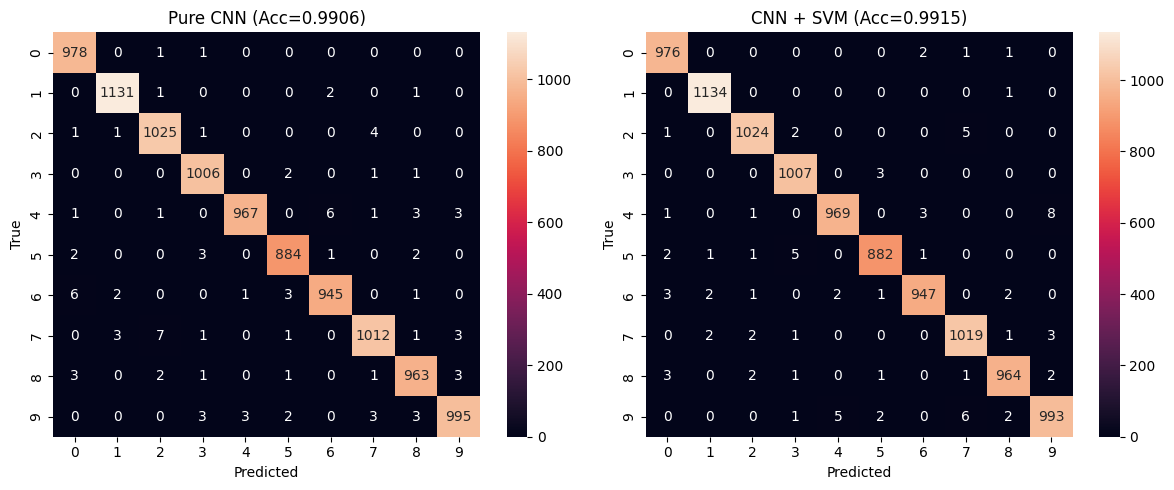
\includegraphics[width=\textwidth]{cnn-svm.png} 
\caption{Confusion matrices for the CNN (left) and CNN+SVM (right)}
\label{fig:confusion_matrix}
\end{figure}

\subsection{t-SNE Plot}
Figure~\ref{fig:tsne} shows that features from different digits form clear clusters. This means the CNN learned features that separate digits well.

\begin{figure}[h!]
\centering
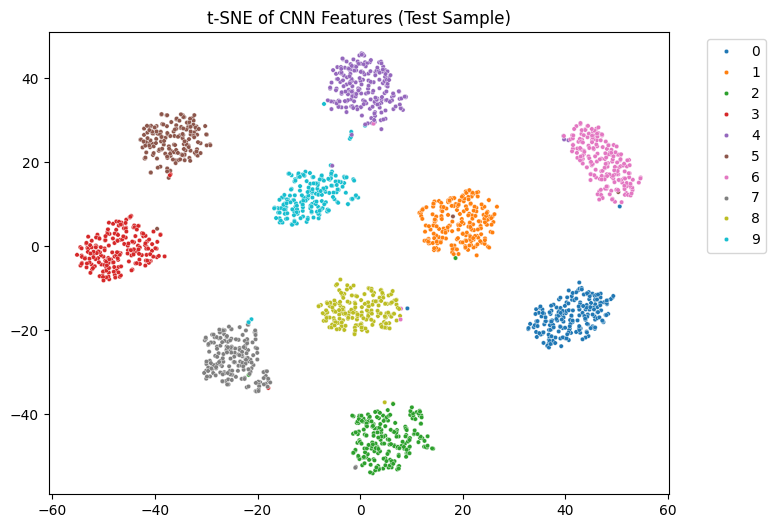
\includegraphics[width=0.7\textwidth]{sne-features.png} 
\caption{t-SNE of CNN features from test images}
\label{fig:tsne}
\end{figure}

\section{Discussion}
Both models performed extremely well. The CNN alone reached 99.06\% accuracy, showing that it can learn complex patterns directly from raw pixels. The hybrid model did slightly better (99.15\%), likely because the features were already well separated, and the SVM’s margin-based classification gave a small boost.

The t-SNE plot supports this: digit clusters are clear and well apart, which is perfect for an SVM. The confusion matrices confirm that both models rarely confuse digits.

\section{Conclusion}
This experiment confirms that a plain CNN is already excellent for MNIST. Adding an SVM on top of the CNN features can improve accuracy slightly. The gain is small, but it shows that in cases where CNN features are easy to separate, an SVM can find an even better decision boundary.

\end{document}